\chapter{量子力学回顾 (QM Review)}\label{ch:qmreview}

本章对量子力学中与散射理论密切相关的数学基础做一个回顾, 并给出散射问题的物理背景. 内容主要参考 Taylor《Scattering Theory》第一、二章. 本章首先用几个典型的实验介绍``散射''在物理学中的中心地位, 随后引入散射理论的基本分类(单道/多道, 时间相关/无关, 相对论/非相对论), 最后系统地复习 Hilbert 空间、Dirac 记号、线性算符、单位算符、厄米共轭、幺正算符、isometric 算符以及态矢量与算符的极限等数学工具. 这些工具会在后续各章中反复使用.

\section{物理学中的量子散射过程}\label{sec:qm-scattering-physics}

散射过程是探索微观物质结构、研究量子物理的最重要的实验手段之一. 直接``看到''微观粒子是不可能的, 我们只能通过让一束粒子去碰撞另一束粒子(或固定的靶), 测量散射后的粒子分布, 从而反推被研究客体的结构与相互作用.

\subsection{Rutherford 的 \texorpdfstring{$\alpha$}{α} 粒子散射实验}

在 Rutherford 的 $\alpha\to$ 金箔散射实验中:
\begin{itemize}
    \item 大多数 $\alpha$ 粒子穿过金箔, 没有偏折;
    \item 少量 $\alpha$ 粒子有比较小角度的偏折, 极少数有非常大角度的偏折.
\end{itemize}
该实验表明原子内部正电荷分布并非均匀, 而是集中在一个很小的、带正电的核(原子核)上. 这一实验奠定了原子核物理的开端, 也是``散射截面''这一概念在物理上获得直接验证的最早例子之一.

\subsection{Franck--Hertz 实验}

电子在水银蒸气中散射—— 原子能级的实验证据. 左边电极发射出电子, 中间两个栅板之间加速, 两栅板之间电压由小变大. 电流开始单调增大, 但每隔约 $4.9\,\mathrm{eV}$ 时突然降低. 解释: 电子与汞蒸气发生非弹性散射, 激发 Hg 的电子到高能级, 能级差 $\sim 4.9\,\mathrm{eV}$. 汞激发态跃迁到基态时放光: $\hbar\omega\sim 4.9\,\mathrm{eV}$, 验证 Einstein 的光量子假说. 反应过程
\begin{equation}
e+\mathrm{Hg}\to \mathrm{Hg}^{*}+e\to \mathrm{Hg}+\gamma+e.
\end{equation}

\subsection{原子核结构与高能散射}

更进一步地, $\alpha$ 粒子轰击 $^{14}\mathrm{N}$ 实现了人工核反应:
\begin{equation}
\alpha+{}^{14}\mathrm{N}\to p+{}^{17}\mathrm{O},
\end{equation}
以及更一般的过程
\begin{equation}
\alpha+N,\quad \alpha+\mathrm{He},\quad \alpha+H,\quad \alpha+N\to p+O \;\text{等}.
\end{equation}

到了高能物理的时代, 散射依然是检验标准模型最直接的工具.
\begin{itemize}
    \item 标准模型理论上要求 $W^{\pm}$ 和 $Z^{0}$ 玻色子, 用于传递弱相互作用. 实验上低能数据外推 $W,Z$ 质量在 $50$--$100\,\mathrm{GeV}$ 之间.
    \item 1981 年, CERN 建成 $\mathrm{S}\bar{p}p\mathrm{S}$, $170\,\mathrm{GeV}$ 的 $p\bar p$ 对撞机. $p,\bar p$ 中的夸克和反夸克碰撞, 可产生中间玻色子 $W,Z$, 衰变为夸克或者轻子, 夸克再演化为 jet, 所以观测最后的横向动量背对背的轻子信号即可作为 $W$ 或 $Z$ 产生的信号.
    \item 1982 年, $W^{\pm}$ 的信号被探测到 ($e+$ missing energy). 1983 年, $Z$ 信号被探测到 ($Z\to e^{+}e^{-}$). 1990 年 $\mathrm{S}\bar p p\mathrm{S}$ 升级到 LEP, 精确测量 $m_W=(81.403\pm 0.029)\,\mathrm{GeV}$, $m_Z=(91.1876\pm 0.0021)\,\mathrm{GeV}$.
    \item 自从 Higgs 粒子被提出后, 人们一直在寻找 Higgs 粒子. CERN LEP 精确测量了 $W,Z$ 粒子的质量, 验证了标准模型的各种过程; 到 2000 年关停, 没有找到 Higgs, 给出 Higgs 质量的下限 $114.4\,\mathrm{GeV}$. Fermilab Tevatron 1995 年找到 top 夸克, 直到 2011 年关停, 排除掉 $147$--$180\,\mathrm{GeV}$ 区间. CERN LHC 2010 年运行, 2012 年, CMS, ATLAS 两个探测器上独立的看到了 Higgs 信号, $m_H=125.11\pm 0.11\,\mathrm{GeV}$. 后续工作验证 Higgs 的各种性质: 自旋, 宇称, 各种衰变模式等.
\end{itemize}

\begin{remark}
LHC 的多级加速链: Linac proton ($50\,\mathrm{MeV}$) $\to$ PSB (Proton synchrotron booster) $1.4\,\mathrm{GeV}$ $\to$ PS $25\,\mathrm{GeV}$ $\to$ SPS $450\,\mathrm{GeV}$ $\to$ LHC $7\,\mathrm{TeV}$. Protons: $v\approx 0.999999991\,c$, 频率 $\geq 11000\,\mathrm{cycles/s}$.
\end{remark}

这些例子说明: 散射不仅是一个可计算的量子力学问题, 它本身就是``实验上可观测''的核心物理量. 接下来我们把视角转回理论, 列出研究散射理论的几种不同方式.

\section{散射理论的不同研究方式}\label{sec:scattering-approaches}

研究散射理论可以从不同维度切入:
\begin{itemize}
    \item \textbf{非相对论 vs.\ 相对论散射}: 我们这门课主要讨论非相对论散射, 即把粒子的运动用 Schr\"odinger 方程描述. 相对论散射(QFT)留待后续课程.
    \item \textbf{单道(single channel) vs.\ 多道(multichannel)散射}: 后面将详细讨论.
    \item \textbf{时间相关(time-dependent) vs.\ 时间无关(time-independent)的描述}: 即用波包的演化来定义散射, 还是直接求定态散射波函数.
\end{itemize}

\subsection{单道散射与多道散射}\label{subsec:single-multi-channel}

\begin{definition}[散射道]
同样的入射态, 可以有不同组散射末态, 每一组末态称为一个\emph{散射道} (channel).
\end{definition}

\begin{itemize}
    \item \emph{单道散射} (single channel scattering): 只有一组散射末态.
    \item \emph{多道散射} (multichannel scattering): 可以有不止一组散射末态.
\end{itemize}

\begin{example}[多道散射]
$\alpha$ 粒子打在 ${}^{14}\mathrm{N}$ 上的可能末态:
\begin{align}
\alpha+{}^{14}\mathrm{N}&\to \alpha+{}^{14}\mathrm{N},\\
                       &\to p+{}^{17}\mathrm{O},\\
                       &\to \alpha+\alpha+{}^{10}\mathrm{B},\\
                       &\;\;\vdots
\end{align}
\end{example}

\begin{example}[单道近似]
低能下的弹性散射, 例如
\begin{equation}
e+p\to e+p,\qquad n+\alpha\to n+\alpha
\end{equation}
即量子力学课程中的``势散射''. 实际上单道散射是一种理想化的近似. 例如 $n$--$\alpha$ collision above $20\,\mathrm{MeV}$ 时, $n$ 会 knock $\alpha$ apart; $e$--$p$ 弹性散射在带电粒子加速时总会伴随 photon 辐射.
\end{example}

\subsection{时间相关与时间无关的散射描述}\label{subsec:td-vs-ti}

\subsubsection{时间无关的表述: 定态散射}

量子力学教科书中的势散射一般用时间无关的方法处理. 以入射动量为 $\mathbf{p}$ 的态为例, 远场行为(asymptotic form)写作
\begin{equation}\label{eq:psip-asymptotic}
\psi^{+}_{\mathbf p}(\mathbf x)\;\xrightarrow{r\to\infty}\;(2\pi)^{-3/2}\Big[\rme^{\rmi\mathbf{p}\cdot\mathbf{x}}+f(E,\theta)\,\frac{\rme^{\rmi p r}}{r}\Big],
\end{equation}
即入射动量为 $\mathbf{p}$ 的粒子束加上散射的球面波, 振幅为 $f(E,\theta)$. 与之对应的微分散射截面定义为
\begin{equation}\label{eq:diff-cross-section}
\frac{\rmd\sigma}{\rmd\Omega}=\frac{\text{scattered flux/solid angle}}{\text{incident flux/area}}=|f(E,\theta)|^{2}.
\end{equation}

这种描述虽然简洁、计算方便, 但存在若干\emph{物理上的疑点}:
\begin{itemize}
    \item 波函数 $\psi^{+}_{\mathbf p}(\mathbf x)$ 是单坐标 $\mathbf x$ 的函数, 描述的是单个粒子, 而非真实实验中的粒子束.
    \item $\psi^{+}_{\mathbf p}$ 不可归一化(它是平面波加球面波, 在 $L^{2}$ 中不存在).
    \item $\psi^{+}_{\mathbf p}$ 是定态(哈密顿量本征态), 不随时间变化; 而真实的碰撞是随时间演化的.
    \item 定义微分截面时分别计算散射流强和入射流强, 实际上忽略了它们之间的干涉.
\end{itemize}

\subsubsection{时间相关的表述}

更``物理''的图像是把散射看作 \emph{free particles $\to$ collision $\to$ free particles}: 远过去自由飞行, 经过一段相互作用区域, 远未来再变成自由粒子. 用可归一化的波包来描述这一过程, 任何具体的波包都可以分解为不同动量的定态 $\psi^{+}_{\mathbf p}$ 的叠加. 因此, 时间相关的描述与时间无关的描述并不矛盾, 而是互为补充. 后续章节会同时使用这两种语言.

\begin{remark}[作业 0]
回顾量子力学, 求解一维有限深方阱
\[V(x)=-V_{0}\;(0<x<a),\qquad V(x)=0\;(\text{otherwise}),\]
波函数中的透射系数和反射系数; 束缚态的能级, 验证束缚态的能级对应透射波系数和反射波系数的极点位置.
\end{remark}

这条注脚式的作业揭示了一个深刻的事实: 散射振幅作为能量的解析函数, 其极点对应于束缚态. 这个结果在后续讨论 $S$ 矩阵解析性质 (第~\ref{ch:analytic}~章) 与共振 (第~\ref{ch:resonance}~章) 时还会反复出现.

\section{波函数与 Hilbert 空间}\label{sec:wf-hilbert}

\subsection{量子态}

\begin{itemize}
    \item 系统的量子态由波函数 $\psi(x)$ 完全描述.
    \item 线性叠加原理: 若 $\psi_1,\psi_2$ 是允许的量子态, 那么 $a\psi_1(x)+b\psi_2(x)$ 也是 ($a,b\in\C$).
    \item 概率解释: $P=\int \rmd^{3}x\,\psi^{*}(x)\psi(x)\geq 0$, 因此波函数应可归一化.
    \item \emph{Proper state}: 可以归一化的态, 它们组成一个线性空间.
    \item \emph{Improper state}: 不可归一化的波函数, 例如平面波
    \begin{align}
        \inn{\mathbf x}{\mathbf p}&=(2\pi)^{-3/2}\rme^{\rmi\mathbf p\cdot\mathbf x},\label{eq:plane-wave-x}\\
        \inn{\mathbf p}{\mathbf p'}&=\delta^{(3)}(\mathbf p-\mathbf p').\label{eq:p-orthogonality}
    \end{align}
    只有 proper states 是物理上可实现的; improper states 只是用来作为基矢展开.
    \item 可观测量(observables) 对应线性厄米算符 (Hermitian operators).
\end{itemize}

对应的数学描述就是 \emph{Hilbert space}.

\subsection{Hilbert 空间}\label{subsec:hilbert-space}

\begin{definition}[Hilbert 空间]
线性复向量空间 $\Hilb$, 维数有限或无穷, 数域 $F=\C$. 内积是映射
\[(\cdot,\cdot):\;\Hilb\times\Hilb\to\C,\;(u,v)\mapsto (u,v),\]
满足:
\begin{enumerate}
    \item \emph{正定性} (positive definite): $(u,u)\in\R_{+}$, 且 $(u,u)=0\Leftrightarrow u=\mathbf 0$.
    \item \emph{线性}: $(u,av_1+bv_2)=a(u,v_1)+b(u,v_2)$, $a,b\in\C$.
    \item \emph{对称性}: $(u,v)^{*}=(v,u)$.
\end{enumerate}
由内积定义\emph{范数}(norm) $\|u\|=\sqrt{(u,u)}$, 由范数定义\emph{度量} $d(u,v)=\|u-v\|$.

\emph{完备性} (completeness): 在上述范数下, 任意 Cauchy 序列 $\{u_n\}$ ($\lim_{m,n\to\infty}d(u_n,u_m)\to 0$) 在 $\Hilb$ 中有极限:
\begin{equation}
\exists u\in\Hilb,\quad \lim_{n\to\infty}\|u_n-u\|=0.
\end{equation}

\emph{可分性} (separable): 存在可数的基矢 $\{u_n\}$, $u_n\in\Hilb$.
\end{definition}

\begin{definition}[稠密子集]
子集 $S\subset\Hilb$, 若对 $\forall v\in\Hilb, \forall \epsilon>0$, 存在 $u\in S$ 使得 $\|u-v\|<\epsilon$, 则称 $S$ 在 $\Hilb$ 中稠密. 此概念可以推广到两个集合之间.
\end{definition}

\begin{remark}
``量子态''与 Hilbert 空间中的矢量是不是一一对应的?  答: 不是. 物理上, 相位整体改变 $\rme^{\rmi\alpha}\ket\psi$ 与 $\ket\psi$ 描述同一个态; 整体非零标量乘子也代表同一个态. 严格说来, 量子态对应于希尔伯特空间中的``射线'' (ray), 即等价类 $\{\lambda\ket\psi:\lambda\in\C\setminus\{0\}\}$. 这一点对后面定义 $S$-矩阵不变性时尤其重要.
\end{remark}

\subsection{Hilbert 子空间}\label{subsec:subhilbert}

\begin{definition}[Hilbert 子空间]
$\Hilb$ 的 Hilbert 子空间 $\mathcal S$ 是 $\Hilb$ 的子集, 它满足 Hilbert 空间定义的所有条件且内积与 $\Hilb$ 上的内积一致.
\end{definition}

\begin{itemize}
    \item $\ket\phi$ 与 $\mathcal S$ 正交: 若对 $\forall u\in\mathcal S$, $\inn{\phi}{u}=0$.
    \item 正交补 $\mathcal S^{\perp}=\{\ket\phi\in\Hilb:\ket\phi\perp \mathcal S\}$.
    \item $\Hilb=\mathcal S\oplus \mathcal S^{\perp}$.
    \item 互相正交的子空间 $\{\mathcal S_i\}$: $\Hilb=\sum_i\oplus \mathcal S_i$, $\Hilb$ is the direct sum of all $\mathcal S_i$.
\end{itemize}

正交分解将在束缚态空间与散射态空间的区分中起核心作用——见后续 Asymptotic Completeness 的讨论.

\subsection{例: \texorpdfstring{$L^{2}(\R)$}{L²(R)} 空间}\label{subsec:L2-example}

\begin{definition}[$L^{2}$ 空间]
模方可积函数空间
\begin{equation}
L^{2}(\R,\rmd x)=\Big\{f:\R\to\C\;\Big|\;\int_{\R}\rmd x\,|f(x)|^{2}<\infty\Big\}.
\end{equation}
零元是``所有积分为零的函数''构成的集合(只在测度为 $0$ 的区域上不为零的函数). 内积
\begin{equation}
(f,g)_{L^{2}}=\int_{\R}\rmd x\,\overline{f(x)}\,g(x),\quad f,g\in L^{2}(\R,\rmd x).
\end{equation}
\end{definition}

它是一个 Hilbert 空间. 几点说明:
\begin{itemize}
    \item 严格地说, $L^{2}$ 中的元素是函数的等价类: 两个函数若仅在测度为零的集合上不同, 则视为相同元素.
    \item Fourier 变换: 动量空间波函数也是 $L^{2}(\R,\rmd p)$ 空间元素,
    \begin{equation}
    \mathcal F:L^{2}(\R,\rmd x)\to L^{2}(\R,\rmd p),\qquad
    f\mapsto \mathcal F f,\quad (\mathcal F f)(p)=\frac{1}{\sqrt{2\pi\hbar}}\int_{\R}\rmd x\,f(x)\,\rme^{-\rmi p x/\hbar}.
    \label{eq:fourier-1d}
    \end{equation}
    Fourier 变换是 $L^{2}$ 上的幺正映射 (Plancherel 定理). 三维形式
    \begin{equation}
    (\mathcal F f)(\mathbf p)=\frac{1}{(2\pi\hbar)^{3/2}}\int_{\R^{3}}\rmd^{3}x\,f(\mathbf x)\,\rme^{-\rmi\mathbf p\cdot\mathbf x/\hbar}.
    \end{equation}
    \item $\delta(x)$, $\rme^{\rmi k x}$ 等不在 $L^{2}$ 中(范数发散), 它们是 improper states, 只在分布意义下存在.
\end{itemize}

\subsection{例: \texorpdfstring{$\ell^{2}(\C)$}{ℓ²(C)} 空间}\label{subsec:l2-example}

\begin{definition}[$\ell^{2}$ 空间]
模方可求和的复序列集合
\begin{equation}
\ell_{2}=\Big\{\vec c=(c_0,c_1,\dots)\;\Big|\;c_n\in\C,\;\sum_{n=0}^{\infty}|c_n|^{2}<\infty\Big\}.
\end{equation}
内积
\begin{equation}
(\vec c,\vec c\,')=\sum_{n=0}^{\infty}c_n^{*}c_n',\qquad \forall \vec c,\vec c\,'\in\ell_2.
\end{equation}
\end{definition}

它构成 Hilbert 空间, 记作 $\ell^{2}$.

\begin{theorem}\label{thm:l2-isomorphism}
$L^{2}$ 与 $\ell^{2}$ 都是可分的 Hilbert 空间. 任意无穷维可分 Hilbert 空间与 $\ell^{2}$ 等价(同构).
\end{theorem}

这个结果是 Riesz--Fischer 定理的一个推论. 物理意义: 不论我们用 $L^{2}$ 还是用谐振子能量本征态构成的 $\ell^{2}$ 序列空间, 它们作为抽象的 Hilbert 空间是同一个对象——这正是 Schr\"odinger 波动力学和 Heisenberg 矩阵力学等价的数学根源.

\section{Dirac 记号}\label{sec:dirac-notation}

物理上常用 Dirac 的 bra-ket 记号. 这一节把它放在 Hilbert 空间和它的对偶空间的语言下严格化.

\begin{itemize}
    \item $\Hilb$ 中的每一个矢量我们用 \emph{Dirac ket} $\ket n$ 表示.
    \item \emph{对偶 Hilbert 空间} $\Hilb^{*}$: 全体有界线性泛函 $f:v\mapsto f(v)\in\C$ 构成的空间, 满足
    \begin{equation}
    \forall u,v\in\Hilb,\quad f(au+bv)=a\,f(u)+b\,f(v).
    \end{equation}
    有界性: $\exists c>0$, $\forall u\in\Hilb$, $|f(u)|\leq c\,\|u\|$. 所有有界线性泛函构成一个线性空间 $\Hilb^{*}$.
    \item $\Hilb\sim \Hilb^{*}$: 内积 $(u,v)$ 定义了一个一一映射 (bijective, one-to-one and onto) $\Hilb\to\Hilb^{*}$ (Riesz 引理):
    \begin{equation}
    \forall u\in\Hilb,\;\; u\mapsto f_u=(u,\cdot).
    \end{equation}
    在对偶空间 $\Hilb^{*}$ 中的矢量表示为 \emph{bra} $\bra u\equiv f_u$.
    \item 内积写为 $\inn{u}{v}=(u,v)$.
\end{itemize}

\begin{remark}
按上面的约定, 内积在第二个变量上线性, 在第一个变量上反线性, 即
\[\inn{u}{a v_1+b v_2}=a\inn{u}{v_1}+b\inn{u}{v_2},\quad \inn{a u_1+b u_2}{v}=a^{*}\inn{u_1}{v}+b^{*}\inn{u_2}{v}.\]
这是物理学家的惯例(Taylor、Sakurai), 与某些数学书中``左线性右反线性''的约定相反, 后续公式都按此约定.
\end{remark}

\section{线性算符}\label{sec:linear-operators}

\begin{definition}[线性算符]
\emph{定义域} $\mathscr D(A)\subset \Hilb$ 是 $\Hilb$ 的子空间. 算符 $A$ 是线性映射 $A:\mathscr D(A)\mapsto \Hilb$, 即对 $\forall u,v\in\mathscr D(A)$, 有 $Au,Av\in\Hilb$,
\begin{equation}
A(\lambda_1 u+\lambda_2 v)=\lambda_1 Au+\lambda_2 Av,\quad \forall \lambda_1,\lambda_2\in\C.
\end{equation}
\end{definition}

关于定义域、值域、有界性、相等等概念:
\begin{itemize}
    \item 算符 $A$ 的定义域 $\mathscr D(A)$ 不一定是整个 $\Hilb$, 不是所有 $Au$ 都有意义. 例: 位置算符 $\hat x$ 在 $L^{2}(\R)$ 中, 仅在 $\{\psi:x\psi\in L^{2}(\R)\}$ 上有定义.
    \item \emph{值域} $\mathscr R(A)$: $u\in\mathscr R(A)$ 表示存在 $v\in\Hilb$, 使得 $Av=u$.
    \item 两个算符 $A,B$ 若 $\mathscr D(A)\subset\mathscr D(B)$, 且 $\forall u\in\mathscr D(A)$, $Au=Bu$, 则记为 $A\subset B$.
    \item \emph{有界线性算符}: $A$ 有界, 即 $\exists M>0, \forall u\in\Hilb$, $\|Au\|\leq M\|u\|$, 此时 $\mathscr D(A)=\Hilb$.
    \item \emph{核} (Kernel) $\mathrm{Ker}(A)=\{\psi\in\mathscr D(A): A\psi=\mathbf 0\}$.
\end{itemize}

\subsection{单射、可逆性}

\begin{definition}[单射 (injective)]
$A$ 是单射: 若 $\forall u,v\in\mathscr D(A)$, $u\neq v$, 则 $Au\neq Av$.
\end{definition}

如果 $A$ 不是单射, 即 $\exists u\neq v$ 使 $Au=Av$, 则 $A$ 是不可逆的. 反之若 $A$ 单射, 则可定义逆算符 $A^{-1}:\mathscr R(A)\mapsto \mathscr D(A)$, 使得 $\forall v\in\mathscr R(A)$, 存在唯一 $u\in\mathscr D(A)$ 满足 $Au=v$, 即
\begin{equation}
A^{-1}v=u,\qquad \mathscr D(A^{-1})=\mathscr R(A),\;\mathscr R(A^{-1})=\mathscr D(A).
\end{equation}

\begin{proposition}\label{prop:invertibility}
线性算符 $A$ 存在逆算符 $A^{-1}$ $\Longleftrightarrow$ $u\neq \mathbf 0\Rightarrow Au\neq \mathbf 0$, 即 $\mathrm{Ker}(A)=\{\mathbf 0\}$.
\end{proposition}

\subsection{单位算符}\label{subsec:identity}

\begin{definition}[单位算符]
单位算符 $I$: 对 $\forall u\in\Hilb$, $I\ket u=\ket u$.
\end{definition}

两个算符相等: $A=B$ 当且仅当 $\mathscr D(A)=\mathscr D(B)$, 且对 $\forall u\in\mathscr D(A)$, $A\ket u=B\ket u$.

\begin{remark}[作业 1]
证明:
\begin{enumerate}
    \item 若 $v\in\Hilb$, 对 $\forall u\in\Hilb$, $\inn{v}{u}=0$, 则 $v=\mathbf 0$.
    \item $v,\tilde v\in\Hilb$, 若对 $\forall u\in\Hilb$, $\inn{v}{u}=\inn{\tilde v}{u}$, 则 $v=\tilde v$.
    \item 对 $\forall u,v\in\Hilb$, $\matel{u}{A}{v}=\inn{u}{v}$, 则 $A=I$.
    \item 两算符 $A=B$ $\Leftrightarrow$ $\mathscr D(A)=\mathscr D(B)$, 且对 $\forall u\in\Hilb,\forall v\in\mathscr D(A)$, $\matel{u}{A}{v}=\matel{u}{B}{v}$.
\end{enumerate}
\end{remark}

下面给出 (1)(2)(3) 的简短证明思路, 它们在后续推导算符等式时反复使用.

\begin{proof*}
(1) 取 $u=v$: $\inn{v}{v}=\|v\|^{2}=0\Rightarrow v=\mathbf 0$.

(2) 由 (1), $\inn{v-\tilde v}{u}=0$ 对一切 $u$ 成立, 故 $v-\tilde v=\mathbf 0$.

(3) 任取 $v\in\Hilb$, 令 $w=A v-v$. 对 $\forall u$, $\inn{u}{w}=\matel{u}{A}{v}-\inn{u}{v}=0$. 由 (1), $w=\mathbf 0$, 即 $A v=v$ 对一切 $v$ 成立, 故 $A=I$.
\end{proof*}

\section{厄米共轭}\label{sec:adjoint}

\subsection{定义}

设 $A$ 的定义域 $\mathscr D(A)$ 在 $\Hilb$ 中稠密(可以稠定即可). 厄米共轭 $\Op A^{\dagger}$ 的定义域:
\begin{equation}
\mathscr D(\Op A^{\dagger})=\Big\{\psi\in\Hilb\;\Big|\; \exists \tilde\psi\in\Hilb,\;\text{s.t.}\;\forall \varphi\in\mathscr D(\Op A),\;\matel{\psi}{\Op A}{\varphi}=\inn{\tilde\psi}{\varphi}\Big\}.
\end{equation}
我们定义 $\Op A^{\dagger}$ 算符
\begin{equation}
\Op A^{\dagger}\ket\psi=\ket{\tilde\psi}.
\end{equation}
$\Op A^{\dagger}$ 也为一线性算符, 称作 $\Op A$ 的厄米共轭算符.

\begin{itemize}
    \item $\mathscr D(\Op A)$ 稠密导致若给定 $\ket\psi$, 则 $\ket{\tilde\psi}$ 唯一. (否则两个不同的 $\tilde\psi,\tilde\psi'$ 给出 $\inn{\tilde\psi-\tilde\psi'}{\varphi}=0$ 对稠密集成立, 由连续性推到全空间, 故二者相等.)
    \item $\mathrm{Ker}(\Op A^{\dagger})=\mathscr R(\Op A)^{\perp}$.
    \item 若 $A\subset B$, 则 $B^{\dagger}\subset A^{\dagger}$.
    \item 若 $A$ 是有界算符, $\mathscr D(A)=\Hilb$, 由 Riesz 引理, $\forall \ket\psi$ 都有唯一的 $\ket{\tilde\psi}$ 满足定义, 所以这类算符 $A$, $\mathscr D(\Op A^{\dagger})=\Hilb$. (例如有界线性算符.)
    \item 对一般的算符, $\mathscr D(\Op A)\neq \mathscr D(\Op A^{\dagger})$.
\end{itemize}

\subsection{对称算符与自伴算符}

\begin{definition}[对称算符]
若 $\forall f,g\in\mathscr D(A)$, $(Af,g)=(f,Ag)$, 则 $A$ 是对称算符 (symmetric), 即 $A\subset A^{\dagger}$.
\end{definition}

\begin{definition}[自伴/厄米算符]
$A$ 是\emph{自伴} (self-adjoint) 算符: $A=A^{\dagger}$, 即 $\mathscr D(\Op A)=\mathscr D(\Op A^{\dagger})$, 且作用相同.
\end{definition}

\begin{remark}
物理学中常说``厄米''有时只指对称, 但只有自伴算符才有完整的实谱和谱定理. 在散射理论中, $\Op H$ 必须是自伴算符, 才能给出幺正的演化算符 $\rme^{-\rmi\Op H t/\hbar}$.
\end{remark}

\begin{remark}[作业 2]
证明:
\begin{enumerate}
    \item $\Op A^{\dagger}$ 也为一线性算符.
    \item 若 $A\subset B$, 即 $\mathscr D(A)\subset\mathscr D(B)$ 且二者作用相同, 则 $B^{\dagger}\subset A^{\dagger}$.
    \item 若 $u\in\mathscr D(A)$, $v\in\mathscr D(A^{\dagger})$, 则 $\matel{Au}{}{v}=\matel{u}{A^{\dagger}}{v}$, 即 $\inn{Au}{v}=\matel{u}{A^{\dagger}}{v}$.
\end{enumerate}
\end{remark}

\section{幺正算符与 Isometric 算符}\label{sec:unitary-isometric}

这一节是本章的核心, 因为整个散射理论的``M\o ller 算符''与``$S$ 算符''都是 isometric 或 unitary 算符.

\subsection{Unitary operator}\label{subsec:unitary}

\begin{definition}[幺正算符]
线性算符 $U$ 称为\emph{幺正算符} (unitary), 若
\begin{enumerate}
    \item 定义域和值域都是整个空间: $\mathscr D(U)=\mathscr R(U)=\Hilb$;
    \item 保内积: $\forall u,v\in\Hilb$, $\inn{Uu}{Uv}=\inn{u}{v}$.
\end{enumerate}
等价地, $\mathscr R(U)=\Hilb$ 且 $\forall u\in\Hilb$, $\|Uu\|=\|u\|$.
\end{definition}

\begin{proposition}\label{prop:unitary-equivalent}
对于满足 $\mathscr D(U)=\mathscr R(U)=\Hilb$ 的线性算符 $U$, ``保内积''与``保 norm''等价.
\end{proposition}

\begin{proof*}
保内积 $\Rightarrow$ 保 norm 显然(取 $u=v$). 反之, 由极化恒等式
\[\inn{u}{v}=\tfrac14\big(\|u+v\|^{2}-\|u-v\|^{2}-\rmi\|u+\rmi v\|^{2}+\rmi\|u-\rmi v\|^{2}\big),\]
可由保 norm 推出保内积.
\end{proof*}

由保内积可得
\begin{equation}
\inn{Uu}{Uv}=\matel{u}{U^{\dagger}U}{v}=\inn{u}{v}\quad\Rightarrow\quad U^{\dagger}U=I.
\end{equation}
又因 $\mathscr R(U)=\Hilb$, 所以 $\forall \phi\in\Hilb$, 存在 $\psi$ 使 $\phi=U\psi$, 故
\begin{equation}
U U^{\dagger}\phi=U U^{\dagger}U\psi=U\psi=\phi\quad\Rightarrow\quad U U^{\dagger}=I.
\end{equation}
所以
\begin{equation}\label{eq:unitary-twoways}
U^{\dagger}U=I=UU^{\dagger}.
\end{equation}
即 $U^{\dagger}=U^{-1}$, 这是幺正算符的最常用判据.

\begin{example}[时间演化]
对于一个保守系统, 若 $\Op H$ 不显含 $t$, $\Op H$ 是自伴算符, 那么时间演化算符
\begin{equation}
U(t)=\rme^{-\rmi\Op H t/\hbar}
\end{equation}
是幺正算符, $\mathscr D(U)=\mathscr R(U)=\Hilb$, $U^{\dagger}(t)U(t)=U(t)U^{\dagger}(t)=I$. 这保证概率守恒.
\end{example}

\begin{remark}[作业 3]
\begin{enumerate}
    \item 证明: 上面``保内积''和``保 norm''是等价的.
\end{enumerate}
\end{remark}

\subsection{Isometric operator}\label{subsec:isometric}

\begin{definition}[Isometric operator]
\begin{itemize}
    \item 定义域是整个空间: $\mathscr D(\Omega)=\Hilb$.
    \item 保 norm: $\forall u\in\Hilb$, $\|\Omega u\|=\|u\|$.
\end{itemize}
\end{definition}

\begin{itemize}
    \item 注意没有要求值域是整个空间, 一般来说 $\mathscr R(\Omega)\neq \Hilb$.
    \item 幺正算符都是 isometric, 但反之不一定成立.
    \item 对于有限维空间, isometric 与幺正没有区别(单射加保 norm 已足够).
    \item 只有在无穷维空间中两者才有区别.
\end{itemize}

\begin{example}[单边平移算符]
取一组基 $\ket 1,\ket 2,\dots$, 定义
\begin{equation}
\Omega\ket n=\ket{n+1},\qquad n\geq 1.
\end{equation}
$\Omega$ 在它的值域 $\mathscr R(\Omega)=\mathrm{span}\{\ket 2,\ket 3,\dots\}$ 上有逆:
\begin{equation}
\Omega^{-1}\ket n=\ket{n-1},\quad n\geq 2,
\end{equation}
然而 $\Omega^{-1}\ket 1$ 没有定义. 故 $\Omega^{-1}\Omega=I$, 但 $\Omega\Omega^{-1}\neq I$, 后者只在 $\mathrm{span}\{\ket 2,\ket 3,\dots\}$ 上为 $I$.
\end{example}

\subsubsection{Isometric 算符的厄米共轭}

对 isometric operator $\Omega$, 一般来说 $\Omega^{\dagger}\neq \Omega^{-1}$, 定义域可能不同. 由保内积:
\begin{equation}
\forall \psi,\chi\in\Hilb,\quad\inn{\Omega\psi}{\Omega\chi}=\matel{\psi}{\Omega^{\dagger}\Omega}{\chi}=\inn{\psi}{\chi},
\end{equation}
我们有 $\Omega^{\dagger}\Omega=I$, 即 $\Omega^{\dagger}\Omega\ket\chi=\ket\chi$, 即对 $\phi\in\mathscr R(\Omega)$, $\Omega^{\dagger}\ket\phi=\Omega^{-1}\ket\phi$.

但是, 若 $\phi\perp\mathscr R(\Omega)$, 对 $\forall \chi\in\Hilb$,
\begin{equation}
\matel{\phi}{\Omega}{\chi}=\matel{\Omega^{\dagger}\phi}{}{\chi}=0,
\end{equation}
所以 $\Omega^{\dagger}\ket\phi=\mathbf 0$. 即 $\mathrm{Ker}\,\Omega^{\dagger}=\mathscr R(\Omega)^{\perp}$.

综合两种情况, $\Omega^{\dagger}$ 的定义域为整个 $\Hilb$:
\begin{equation}\label{eq:omega-dagger-def}
\Omega^{\dagger}\ket\chi=\begin{cases}\Omega^{-1}\ket\chi,& \ket\chi\in\mathscr R(\Omega),\\ \mathbf 0,& \ket\chi\in\mathscr R(\Omega)^{\perp},\end{cases}
\end{equation}
即 $\mathscr D(\Omega^{-1})=\mathscr R(\Omega)$.

\subsubsection{图像化对比}

幺正算符 $U$ 给出 $\Hilb=\mathscr D(U)$ 与 $\Hilb=\mathscr R(U)$ 之间的一一对应: 每一个 $\ket\psi$ 都有唯一的像 $\ket{\psi'}$, 每一个 $\ket{\phi'}$ 都是某唯一 $\ket\phi$ 的像.

isometric 算符 $\Omega$ 则是把 $\Hilb$ ``等距''映射到自身的一个真子空间(可能是真子集)中, 像在物理上``往后传一格''. 这正是 M\o ller 算符 $\Omega_{\pm}$ 的典型行为: 它们把自由 Hilbert 空间 $\Hilb$ 嵌入到全 Hilbert 空间的散射子空间 $\mathscr R(\Omega_\pm)\subset\Hilb$ 中, 一般来说不覆盖整个 $\Hilb$ (因为可能存在束缚态), 故是 isometric 但不是 unitary.

\section{矢量与算符的极限}\label{sec:limits}

在散射理论里我们经常要考虑 $t\to\pm\infty$ 时态和算符的极限. 这一节区分``强极限''和``弱极限'', 它们对应不同的物理意义.

\subsection{矢量的极限}

\begin{definition}[强极限]
$\ket{\psi_t}$ 在 $t\to\infty$ 时\emph{强收敛}于极限矢量 $\ket\psi$, 当且仅当
\begin{equation}
\|\psi_t-\psi\|\xrightarrow{t\to\infty}0.
\end{equation}
\end{definition}

\begin{definition}[弱极限]
$\ket{\psi_t}$ 在 $t\to\infty$ 时\emph{弱收敛}于 $\ket\psi$, 当且仅当
\begin{equation}
\lim_{t\to\infty}\inn{\chi}{\psi_t}=\inn{\chi}{\psi},\quad \forall \ket\chi\in\Hilb.
\end{equation}
\end{definition}

强收敛 $\Rightarrow$ 弱收敛: 由 Cauchy--Schwarz 不等式 $|\inn{\chi}{\psi_t-\psi}|\leq\|\chi\|\|\psi_t-\psi\|\to 0$. 反之不一定成立: 弱极限存在的话不一定存在强极限.

\begin{example}[自由波包]
取自由波包 $\ket{\psi_0}$ ($\|\psi_0\|=1$), 随时间演化 $\ket{\psi_t}=\rme^{-\rmi\Op H_0 t/\hbar}\ket{\psi_0}$, 在空间会弥散开来. 可以证明
\begin{equation}
\lim_{t\to\infty}\inn{\mathbf x}{\psi_t}=\inn{\mathbf x}{\mathbf 0}=0,
\end{equation}
即坐标空间任一点的概率振幅趋向 $0$, 故 $\ket{\psi_t}$ 弱收敛到 $\mathbf 0$. 但是
\begin{equation}
\|\psi_t-\mathbf 0\|=\|\psi_t\|=1,
\end{equation}
故没有强极限.
\end{example}

物理上, 强极限意味着 $t\to\infty$ 时 $\psi_t$ 与 $\psi$ 整体上``难以区分'' (整个范数都趋同), 这是散射理论中``渐进自由''应有的定义. 弱极限太弱, 不足以保证物理意义.

\subsection{Cauchy 判据}

数列的 Cauchy 判据: $\exists a, \lim_{t\to\infty}|a_t-a|=0\Leftrightarrow \lim_{t,t'\to\infty}|a_t-a_{t'}|=0$.

在 $\Hilb$ 中也有类似定理:
\begin{equation}
\exists \psi\in\Hilb,\;\lim_{t\to\infty}\|\psi_t-\psi\|=0\;\Longleftrightarrow\;\lim_{t,t'\to\infty}\|\psi_t-\psi_{t'}\|=0.
\end{equation}

进一步, 如果
\begin{equation}\label{eq:integral-state}
\ket{\psi_t}=\int_a^t\rmd\tau\,\ket{\psi_\tau},
\end{equation}
$t\to\infty$ 时若收敛, 需要
\[\lim_{t,t'\to\infty}\Big\|\int_t^{t'}\rmd\tau\,\ket{\psi_\tau}\Big\|=0.\]
若 $\lim_{t,t'\to\infty}\int_t^{t'}\rmd\tau\,\|\psi_\tau\|=0$, 那么上式一定成立, 也就是当 $\lim_{t\to\infty}\int_0^t\rmd\tau\,\|\psi_\tau\|<\infty$ 时 $\ket{\psi_t}$ 有极限. 这一估计在证明 M\o ller 算符存在时反复出现:只要``相互作用项的范数''可积, 就保证 M\o ller 算符的强极限存在.

\subsection{算符的极限}

\begin{definition}[算符的弱收敛]
$\lim_{t\to\infty}\matel{\psi}{A_t}{\chi}=\matel{\psi}{A}{\chi}$, 对 $\forall \ket\psi,\ket\chi\in\Hilb$.
\end{definition}

\begin{definition}[算符的强收敛]
$\forall \ket\chi\in\Hilb$, $\exists\ket{\phi_\chi}$ 使
\begin{equation}
\lim_{t\to\infty}\big\|A_t\ket\chi-\ket{\phi_\chi}\big\|=0.
\end{equation}
定义算符 $A$ : $\forall \ket\chi$, $A\ket\chi\equiv \ket{\phi_\chi}$, $\lim_{t\to\infty}A_t\equiv A$.
\end{definition}

后面我们要用到的是\emph{算符的强极限}.

\subsection{Isometric 极限可能不再是幺正}

假设 $U_t$ 都是幺正算符, 且对 $\forall \ket\psi$ 强收敛
\begin{equation}
U_t\ket\psi\to \Omega\ket\psi.
\end{equation}
由于范数在强极限下连续:
\begin{equation}
\|\Omega\psi\|=\lim_{t\to\infty}\|U_t\psi\|=\|\psi\|,
\end{equation}
所以 $\Omega$ 是 isometric 的: $\Omega^{\dagger}\Omega=I$. 但是 $\Omega\Omega^{\dagger}=I$ 一般不一定成立.

\begin{remark}[物理意义]
M\o ller 算符 $\Omega_{\pm}$ 的定义正是
\[\Omega_{\pm}=\lim_{t\to\mp\infty}\rme^{\rmi\Op H t/\hbar}\rme^{-\rmi\Op H_0 t/\hbar},\]
其中 $\rme^{\rmi\Op H t/\hbar}$ 与 $\rme^{-\rmi\Op H_0 t/\hbar}$ 都是幺正算符, 但这一极限是\emph{强极限}, 一般而言只能保证 $\Omega_\pm$ 是 isometric 的, 而非 unitary 的. 它的值域 $\mathscr R(\Omega_\pm)$ 即所谓``散射态子空间''. 当且仅当散射态张满 $\Hilb$ 的束缚态正交补时(\emph{asymptotic completeness}), $\Omega_\pm$ 才是幺正的; 这一深层数学性质正是后续章节``$S$ 算符是幺正的''的来源, 并将在第~\ref{sec:limits} 节及以后多次回顾.
\end{remark}

\section{自由演化算符与自由传播子}\label{sec:qm-free-propagator}

在散射理论中, 自由 Hamiltonian
\begin{equation}\label{eq:qm-H0-def}
\Op H_0=\frac{\Op{\mathbf p}^{2}}{2m}
\end{equation}
扮演核心角色: 散射过程的渐进态由 $\rme^{-\rmi\Op H_0 t/\hbar}$ 演化, M\o{}ller 算符的极限收敛性也归结于自由演化下波包的弥散行为. 本节给出 $\rme^{-\rmi\Op H_0 t/\hbar}$ 在动量空间和坐标空间的显式形式, 并用它讨论自由波包的弥散.

\subsection{动量空间中的自由演化算符}

由于 $\Op H_0$ 与 $\Op{\mathbf p}$ 对易, 在动量表象中自由演化是\emph{逐点相位}:
\begin{equation}\label{eq:qm-U0-momentum}
\bigl(\rme^{-\rmi\Op H_0 t/\hbar}\psi\bigr)(\mathbf p)
=\rme^{-\rmi p^{2} t/(2m\hbar)}\,\psi(\mathbf p),
\end{equation}
其中 $p\equiv|\mathbf p|$. 因此
\begin{equation}\label{eq:qm-p-matel}
\matel{\mathbf p}{\rme^{-\rmi\Op H_0 t/\hbar}}{\mathbf p'}
=\rme^{-\rmi p^{2} t/(2m\hbar)}\,\delta^{(3)}(\mathbf p-\mathbf p').
\end{equation}
显然 $\rme^{-\rmi\Op H_0 t/\hbar}$ 是幺正算符, $\mathscr D=\mathscr R=\Hilb$, 且
\begin{equation}
\bigl\|\rme^{-\rmi\Op H_0 t/\hbar}\psi\bigr\|_{L^{2}(\rmd^{3}p)}
=\|\psi\|_{L^{2}(\rmd^{3}p)}.
\end{equation}
这说明: 在动量空间, 自由演化只改变波函数的相位, 不改变其模; 因此动量分布 $|\psi(\mathbf p)|^{2}$ 是\emph{严格守恒量}. 这一性质在后面分析散射截面时会反复用到.

\subsection{坐标空间中的自由传播子}

通过 Fourier 变换可以得到坐标空间的传播子. 对 $\psi(\mathbf x,t)\equiv\inn{\mathbf x}{\rme^{-\rmi\Op H_0 t/\hbar}\psi}$ 插入完备性
\begin{align}
\psi(\mathbf x,t)
&=\int\rmd^{3}p\,\inn{\mathbf x}{\mathbf p}\rme^{-\rmi p^{2} t/(2m\hbar)}\inn{\mathbf p}{\psi}\nonumber\\
&=\int\rmd^{3}x'\,K_{0}(\mathbf x,\mathbf x';t)\,\psi(\mathbf x',0),
\end{align}
其中自由传播子 (free propagator) 为 Gauss 积分
\begin{equation}\label{eq:qm-free-propagator}
K_{0}(\mathbf x,\mathbf x';t)
=\inn{\mathbf x}{\rme^{-\rmi\Op H_0 t/\hbar}|\mathbf x'}
=\Big(\frac{m}{2\pi\rmi\hbar t}\Big)^{3/2}
\exp\!\Big[\frac{\rmi m\,|\mathbf x-\mathbf x'|^{2}}{2\hbar t}\Big].
\end{equation}
推导: 把 $\inn{\mathbf x}{\mathbf p}=(2\pi\hbar)^{-3/2}\rme^{\rmi\mathbf p\cdot\mathbf x/\hbar}$ 代入, 配方
\[\frac{p^{2}}{2m\hbar}t-\frac{(\mathbf x-\mathbf x')\cdot\mathbf p}{\hbar}
=\frac{t}{2m\hbar}\Big(\mathbf p-\frac{m(\mathbf x-\mathbf x')}{t}\Big)^{2}-\frac{m|\mathbf x-\mathbf x'|^{2}}{2\hbar t},\]
再做三维 Fresnel 积分即得 \eqref{eq:qm-free-propagator}.

\begin{remark}
$K_0(\mathbf x,\mathbf x';t)$ 在 $t\to 0$ 时是 $\delta^{(3)}(\mathbf x-\mathbf x')$ 的振荡逼近: $|K_0|=(m/2\pi\hbar|t|)^{3/2}$, 任一固定点处的 $|K_0|$ 随 $|t|^{-3/2}$ 衰减. 这一 $|t|^{-3/2}$ 因子正是 Taylor 在论证 M\o{}ller 算符存在性时反复用到的``三维波包弥散率''.
\end{remark}

\subsection{自由传播子的群性质}

由 $\rme^{-\rmi\Op H_0 t/\hbar}$ 的指数形式立即得到
\begin{equation}\label{eq:qm-K0-group}
K_{0}(\mathbf x,\mathbf x';t_1+t_2)=\int\rmd^{3}y\,K_{0}(\mathbf x,\mathbf y;t_2)K_{0}(\mathbf y,\mathbf x';t_1),
\end{equation}
即 Chapman--Kolmogorov 方程, 这是 Feynman 路径积分``切片''的源头. 此外
\begin{equation}
K_{0}(\mathbf x,\mathbf x';-t)=\overline{K_{0}(\mathbf x,\mathbf x';t)},\qquad
K_{0}(\mathbf x,\mathbf x';t)=K_{0}(\mathbf x',\mathbf x;t),
\end{equation}
分别对应时间反演对称性与坐标对称性.

\section{自由波包的弥散与渐进零点}\label{sec:qm-spreading}

\subsection{Gauss 波包的精确演化}\label{subsec:qm-gauss}

考虑三维 Gauss 波包
\begin{equation}\label{eq:qm-gauss-init}
\psi_{0}(\mathbf x)=\frac{1}{(\pi\xi^{2})^{3/4}}\,\rme^{-(\mathbf x-\mathbf a)^{2}/(2\xi^{2})}\,\rme^{\rmi\mathbf p_{0}\cdot\mathbf x/\hbar},
\end{equation}
中心位置 $\mathbf a$, 中心动量 $\mathbf p_{0}$, 宽度 $\xi$. 在自由演化下波函数保持 Gauss 形式:
\begin{empheq}[box=\fbox]{equation}\label{eq:qm-gauss-evolve}
|\psi_{t}(\mathbf x)|^{2}=\Big(1+\frac{\hbar^{2} t^{2}}{m^{2}\xi^{4}}\Big)^{-3/2}\frac{1}{(\pi\xi^{2})^{3/2}}\exp\!\Big[-\frac{(\mathbf x-\mathbf a-\mathbf v_{0}t)^{2}}{\xi^{2}+\hbar^{2}t^{2}/(m^{2}\xi^{2})}\Big],
\end{empheq}
其中 $\mathbf v_{0}=\mathbf p_{0}/m$. 几点观察:
\begin{itemize}
    \item 中心以\emph{群速度} $\mathbf v_{0}=\mathbf p_{0}/m$ 匀速直线运动;
    \item 宽度 $\xi(t)=\sqrt{\xi^{2}+\hbar^{2}t^{2}/(m^{2}\xi^{2})}\xrightarrow{|t|\to\infty}\hbar|t|/(m\xi)$, 即长时间下\emph{线性}变宽;
    \item 模方峰值高度 $\sim |t|^{-3}$, 三维体积守恒($\int\rmd^{3}x|\psi|^{2}=1$);
    \item 任一\emph{固定坐标点} $\mathbf x$ 处 $|\psi_{t}(\mathbf x)|^{2}\to 0$ 以 $|t|^{-3}$ 速率, 故 $|\psi_{t}(\mathbf x)|\to 0$ 以 $|t|^{-3/2}$ 速率.
\end{itemize}
这正是 Taylor (1972) eq.~(2.8) 中用到的``$t^{-3/2}$ 弥散率''.

\subsection{Riemann--Lebesgue 引理与弱极限}\label{subsec:qm-RL}

更一般的(非 Gauss) 情形可以借助 Riemann--Lebesgue 引理. 设 $\hat\psi(\mathbf p)=\inn{\mathbf p}{\psi}\in L^{1}(\R^{3})\cap L^{2}(\R^{3})$, 则
\begin{equation}\label{eq:qm-RL-statement}
\psi_{t}(\mathbf x)=\frac{1}{(2\pi\hbar)^{3/2}}\int\rmd^{3}p\,\hat\psi(\mathbf p)\,\rme^{\rmi\mathbf p\cdot\mathbf x/\hbar}\rme^{-\rmi p^{2}t/(2m\hbar)}\xrightarrow{|t|\to\infty}0
\end{equation}
对每一个固定的 $\mathbf x$ 成立. 直观理由是: 当 $|t|$ 很大时, 相位 $-p^{2}t/(2m\hbar)$ 对 $\mathbf p$ 的振荡变得极快, $\rme^{-\rmi p^{2}t/(2m\hbar)}$ 与缓变包络 $\hat\psi(\mathbf p)$ 之乘积的积分趋于零(经典的 Riemann--Lebesgue 论证).

\begin{theorem}[Riemann--Lebesgue]\label{thm:qm-riemann-lebesgue}
若 $f\in L^{1}(\R^{n})$, 则 $\hat f(\mathbf k)\to 0$ 当 $|\mathbf k|\to\infty$.
\end{theorem}

由此可推出: \emph{对任意 $\psi\in L^{2}\cap L^{1}$, 自由演化 $\rme^{-\rmi\Op H_0 t/\hbar}\psi$ 在弱意义上趋于零, 但范数恒为 $\|\psi\|$, 故无强极限.} 这正是第~\ref{sec:limits} 节中提到的 ``弱收敛 $\not\Rightarrow$ 强收敛'' 在自由演化下最重要的实例.

\subsection{驻定相位法与渐进波形}\label{subsec:qm-stationary-phase}

要看清\emph{在 $\mathbf x=\mathbf v t$ 沿群速度方向}波函数的衰减, 需要驻定相位法. 把
\begin{equation}
\psi_{t}(\mathbf x)=\frac{1}{(2\pi\hbar)^{3/2}}\int\rmd^{3}p\,\hat\psi(\mathbf p)\rme^{\rmi\Phi(\mathbf p;\mathbf x,t)/\hbar},\quad
\Phi(\mathbf p;\mathbf x,t)=\mathbf p\cdot\mathbf x-\frac{p^{2}}{2m}t,
\end{equation}
驻定相位条件
\begin{equation}\label{eq:qm-stationary-condition}
\nabla_{\mathbf p}\Phi=\mathbf x-\frac{\mathbf p}{m}t=\mathbf 0\;\Longrightarrow\;\mathbf p_{*}=\frac{m\mathbf x}{t}.
\end{equation}
即在大 $|t|$ 下, 坐标空间点 $\mathbf x$ 处的波函数主要由动量 $\mathbf p_{*}=m\mathbf x/t$ 附近的动量分量贡献. 这一``经典对应''是把动量分布 $|\hat\psi(\mathbf p)|^{2}$ 解读为``某动量分量的概率密度''的物理依据.

\begin{theorem}[驻定相位法, 多维]\label{thm:qm-stationary-phase}
若 $\Phi:\R^{n}\to\R$ 在 $\mathbf p_{*}$ 处有非简并临界点, $\det\partial^{2}\Phi/\partial p_i\partial p_j\big|_{\mathbf p_{*}}\neq 0$, 那么
\begin{equation}
\int\rmd^{n}p\,a(\mathbf p)\rme^{\rmi\lambda\Phi(\mathbf p)}\sim
a(\mathbf p_{*})\Big(\frac{2\pi}{\lambda}\Big)^{n/2}\frac{\rme^{\rmi\sigma\pi/4}}{\sqrt{|\det\Phi''(\mathbf p_{*})|}}\rme^{\rmi\lambda\Phi(\mathbf p_{*})}+O(\lambda^{-n/2-1})
\end{equation}
当 $\lambda\to\infty$, 其中 $\sigma$ 是 Hessian 矩阵 $\Phi''(\mathbf p_{*})$ 正负本征值数的差.
\end{theorem}

应用到自由波包: $\Phi=\mathbf p\cdot\mathbf x-p^{2}t/(2m)$, $\Phi''=-(t/m)\,I_{3}$, $\det\Phi''=-(t/m)^{3}$, 取 $\lambda=1/\hbar$ 并设 $\mathbf x=\mathbf v t$, 得
\begin{equation}\label{eq:qm-asymp-wave}
\psi_{t}(\mathbf v t)\sim \Big(\frac{m}{\rmi\hbar t}\Big)^{3/2}\hat\psi(m\mathbf v)\,\rme^{\rmi m v^{2} t/(2\hbar)}\quad (|t|\to\infty).
\end{equation}
这正是``在自由飞行轨迹 $\mathbf x=\mathbf v t$ 上, 波函数振幅按 $|t|^{-3/2}$ 衰减, 且形状由动量空间波包 $\hat\psi(m\mathbf v)$ 决定''的精确表述. 它是后续章节给出散射波 ``$\rme^{\rmi p r}/r$'' 在三维渐进波展开中物理意义的关键工具(参见第~\ref{ch:Smat1P}, \ref{ch:cross} 章).

\section{自由 Green 函数与解析延拓}\label{sec:qm-free-green}

自由 Hamiltonian $\Op H_0$ 的\emph{预解算符} (resolvent) 定义为
\begin{equation}\label{eq:qm-G0-def}
\Op G_{0}(z)=(z-\Op H_{0})^{-1},\qquad z\in\C\setminus[0,\infty).
\end{equation}
它在散射理论中扮演的角色相当于 Lippmann--Schwinger 方程中的``自由 Green 算符''(见第~\ref{ch:green} 章).

\subsection{动量表象}

由于 $\Op H_0$ 在动量表象中是乘子算符 $p^{2}/(2m)$,
\begin{equation}\label{eq:qm-G0-p}
\matel{\mathbf p}{\Op G_{0}(z)}{\mathbf p'}=\frac{\delta^{(3)}(\mathbf p-\mathbf p')}{z-p^{2}/(2m)}.
\end{equation}
$\Op G_{0}(z)$ 作为 $z$ 的算符值函数, 在 $z\notin[0,\infty)$ 时有界(故有逆), 在 $[0,\infty)$ 上有谱(连续谱)切割.

\subsection{坐标表象的显式公式}

对 $z=k^{2}\hbar^{2}/(2m)+\rmi 0^{+}$ (即从上半 $z$ 平面靠近正实轴, 写成能量 $E=\hbar^{2}k^{2}/(2m)$ 的形式, $k>0$) 有
\begin{equation}\label{eq:qm-G0-x}
\matel{\mathbf x}{\Op G_{0}(E+\rmi 0^{+})}{\mathbf x'}=-\frac{2m}{\hbar^{2}}\frac{1}{4\pi}\frac{\rme^{\rmi k|\mathbf x-\mathbf x'|}}{|\mathbf x-\mathbf x'|},
\end{equation}
即外向球面波 (outgoing) Green 函数. 取 $z=E-\rmi 0^{+}$ 则得内向球面波 (incoming) 的 $\rme^{-\rmi k r}/r$. 这正是定态散射方程 \eqref{eq:psip-asymptotic} 中``入射平面波 $+$ 球面散射波''形式的算符根源.

\subsection{Green 函数与时间演化}

$\Op G_{0}(z)$ 与自由演化算符通过 Laplace 变换相联系:
\begin{equation}\label{eq:qm-laplace}
\Op G_{0}(z)=\frac{1}{\rmi\hbar}\int_{0}^{\infty}\rmd t\,\rme^{\rmi z t/\hbar}\rme^{-\rmi\Op H_{0}t/\hbar},\qquad \mathrm{Im}\,z>0,
\end{equation}
即解析延拓与时间演化之间``半边 Fourier 对偶''. 这一关系后面会推广到全 Hamiltonian 的 Green 算符 $\Op G(z)=(z-\Op H)^{-1}$.

\section{例题 (Examples)}\label{sec:qm-examples}

\begin{example}[一维 Gauss 波包的精确演化]\label{ex:qm-1d-gauss}
取一维初态
\begin{equation}
\psi_{0}(x)=\frac{1}{(\pi\xi^{2})^{1/4}}\rme^{-x^{2}/(2\xi^{2})}\rme^{\rmi p_{0}x/\hbar},
\end{equation}
则 $\hat\psi_{0}(p)=(\xi^{2}/\pi)^{1/4}\hbar^{-1/2}\rme^{-(p-p_{0})^{2}\xi^{2}/(2\hbar^{2})}$. 由 \eqref{eq:qm-U0-momentum},
\begin{equation}
\hat\psi_{t}(p)=\hat\psi_{0}(p)\rme^{-\rmi p^{2} t/(2m\hbar)}.
\end{equation}
回到坐标空间, 配方做 Gauss 积分得
\begin{equation}\label{eq:qm-gauss-1d-x}
\psi_{t}(x)=\frac{1}{[\pi(\xi^{2}+\rmi\hbar t/m)^{2}/\xi^{2}]^{1/4}}\exp\!\Big[-\frac{(x-v_{0}t)^{2}}{2(\xi^{2}+\rmi\hbar t/m)}+\frac{\rmi p_{0}(x-v_{0}t/2)}{\hbar}\Big].
\end{equation}
取模方
\begin{equation}\label{eq:qm-gauss-1d-mod}
|\psi_{t}(x)|^{2}=\frac{1}{\sqrt{\pi}\,\xi(t)}\exp\!\Big[-\frac{(x-v_{0}t)^{2}}{\xi(t)^{2}}\Big],\quad \xi(t)\equiv\sqrt{\xi^{2}+\frac{\hbar^{2}t^{2}}{m^{2}\xi^{2}}}.
\end{equation}
\textbf{物理观察:}
\begin{itemize}
    \item 中心位置 $\langle x\rangle_{t}=v_{0}t$, 群速度 $v_{0}=p_{0}/m$ 与经典粒子一致;
    \item 位置不确定度 $\Delta x(t)=\xi(t)/\sqrt{2}$, 当 $|t|\to\infty$ 时 $\Delta x\sim\hbar|t|/(\sqrt{2}m\xi)$;
    \item 动量不确定度 $\Delta p=\hbar/(\sqrt{2}\xi)$ 守恒(因为 $\Op H_{0}$ 与 $\Op p$ 对易);
    \item 在 $t=0$ 时 $\Delta x\Delta p=\hbar/2$, \emph{饱和}测不准关系; 在 $t\neq 0$ 时不再饱和;
    \item 任意固定 $x$ 点 $|\psi_{t}(x)|^{2}\sim |t|^{-1}\to 0$, 这是一维的 Riemann--Lebesgue 衰减率.
\end{itemize}

也可以验证: 对 \eqref{eq:qm-gauss-1d-x} 直接用 \eqref{eq:qm-free-propagator} 一维形式
\[K_{0}^{(1)}(x,x';t)=\sqrt{\frac{m}{2\pi\rmi\hbar t}}\exp\!\Big[\frac{\rmi m(x-x')^{2}}{2\hbar t}\Big],\]
做 Gauss 积分 $\int\rmd x' K_{0}^{(1)}\psi_{0}(x')$ 得到同样结果.
\end{example}

\begin{example}[测不准关系的饱和]\label{ex:qm-uncertainty}
对一维 Gauss 包络 $\psi(x)=(\pi\xi^{2})^{-1/4}\rme^{-x^{2}/(2\xi^{2})}$, 计算
\begin{align}
\langle x\rangle &=0,\quad \langle x^{2}\rangle=\frac{\xi^{2}}{2}\;\Rightarrow\; \Delta x=\frac{\xi}{\sqrt 2};\\
\langle p\rangle &=0,\quad \langle p^{2}\rangle=\frac{\hbar^{2}}{2\xi^{2}}\;\Rightarrow\; \Delta p=\frac{\hbar}{\sqrt 2\,\xi},
\end{align}
故 $\Delta x\,\Delta p=\hbar/2$, 取等. 这证实了\emph{Gauss 波包是 Heisenberg 测不准关系的饱和态}, 是``最经典''的量子态. 在散射初态制备时, Gauss 形状是常用模型选择.

进一步, 由 \eqref{eq:qm-gauss-1d-mod} 我们有
\[\Delta x(t)\,\Delta p=\frac{\hbar}{2}\sqrt{1+\frac{\hbar^{2}t^{2}}{m^{2}\xi^{4}}}\geq \frac{\hbar}{2},\]
即\emph{自由演化使 Gauss 波包脱离测不准饱和态; 弥散是不可逆的、量子相干的现象}.
\end{example}

\begin{example}[自由波包的远场极限——驻定相位法验证]\label{ex:qm-stationary}
对一维 Gauss \eqref{eq:qm-gauss-init} (取 $a=0$), 直接由 \eqref{eq:qm-gauss-1d-x} 取 $|t|\to\infty$ 极限可得
\begin{equation}
\psi_{t}(x)\simeq \sqrt{\frac{m}{\rmi\hbar t}}\,\hat\psi_{0}(p_{*})\rme^{\rmi p_{*}^{2}t/(2m\hbar)},\quad p_{*}=\frac{mx}{t},
\end{equation}
这与驻定相位法预言 \eqref{eq:qm-asymp-wave}(一维形式 $|t|^{-1/2}$) 完全吻合, 进一步证实了``长时间下波函数主要由动量 $p_{*}=mx/t$ 的分量构成''的物理图像.
\end{example}

\section{数值实验：自由高斯波包的演化}\label{sec:numexp-ch00}

\subsection*{问题}
本节我们用一个最简洁的数值实验把第~\ref{sec:qm-review-summary} 节之前讨论的自由演化算符 $\Op U_{0}(t)=\rme^{-\rmi\Op H_{0}t/\hbar}$ 落到具体计算上: 取自然单位 $\hbar=m=1$, 选初始 Gauss 波包
\begin{equation*}
\psi(x,0)=(\pi\sigma^{2})^{-1/4}\exp\!\Bigl[-\frac{(x-x_{0})^{2}}{2\sigma^{2}}+\rmi p_{0}x\Bigr],\qquad x_{0}=-10,\ p_{0}=2,\ \sigma=1,
\end{equation*}
并数值地求出 $\psi(x,t)$ 在 $t\in\{0,5,10,15\}$ 的形状.

我们关心三件事: (i) 波包中心是否按照 $\langle x\rangle_{t}=x_{0}+p_{0}t$ 经典自由运动? (ii) 坐标方差 $\Delta x(t)$ 是否如理论预言那样线性弥散, 而动量方差 $\Delta p$ 严格守恒? (iii) Heisenberg 不等式 $\Delta x\,\Delta p\ge 1/2$ 是否在初始 ($t=0$) 时被饱和, 之后单调远离下界?

\subsection*{算法}
由于 $\Op H_{0}$ 在动量表象下是逐点乘法算符 $p^{2}/2$, 自由演化在动量空间为一个相位:
\begin{equation*}
\widetilde\psi(p,t)=\widetilde\psi(p,0)\,\rme^{-\rmi p^{2}t/2}.
\end{equation*}
据此实现的算法仅有三步: (1) 对离散坐标网格上的 $\psi(x,0)$ 做正向 FFT 得到 $\widetilde\psi(p,0)$; (2) 逐点乘以相位 $\rme^{-\rmi p^{2}t/2}$; (3) 逆向 FFT 回到坐标空间. 与有限差分或 Crank--Nicolson 不同, 该方案在数值上是精确的 (除浮点截断外不引入时间步误差), 故称为``谱方法''或``Fourier split-step 的零势限'’. 期望值 $\Delta x,\Delta p$ 通过对 $|\psi(x,t)|^{2}$ 与 $|\widetilde\psi(p,t)|^{2}$ 的离散求和直接计算.

\subsection*{Python 实现}
\lstinputlisting[language=Python,caption={\texttt{code/ch00\_wavepacket.py}}]{code/ch00_wavepacket.py}

\subsection*{结果}
\begin{figure}[!htbp]
    \centering
    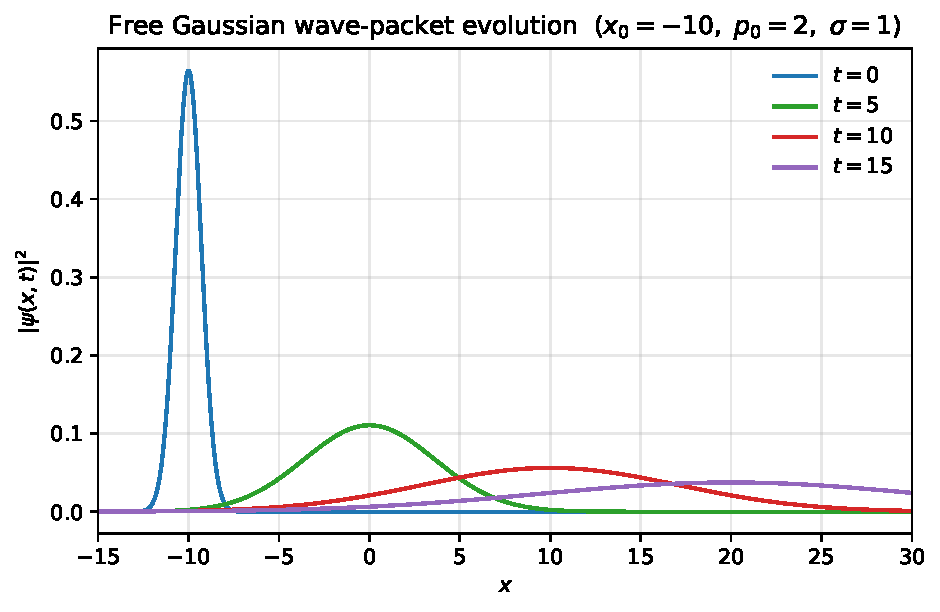
\includegraphics[width=0.9\linewidth]{ch00_wavepacket}
    \caption{$|\psi(x,t)|^{2}$ 在 $t=0,5,10,15$ 的快照. 波包中心严格沿 $\langle x\rangle_{t}=x_{0}+p_{0}t$ 平移, 同时高度下降、宽度增大——这就是``自由弥散''.}
    \label{fig:numexp-ch00}
\end{figure}
\begin{figure}[!htbp]
    \centering
    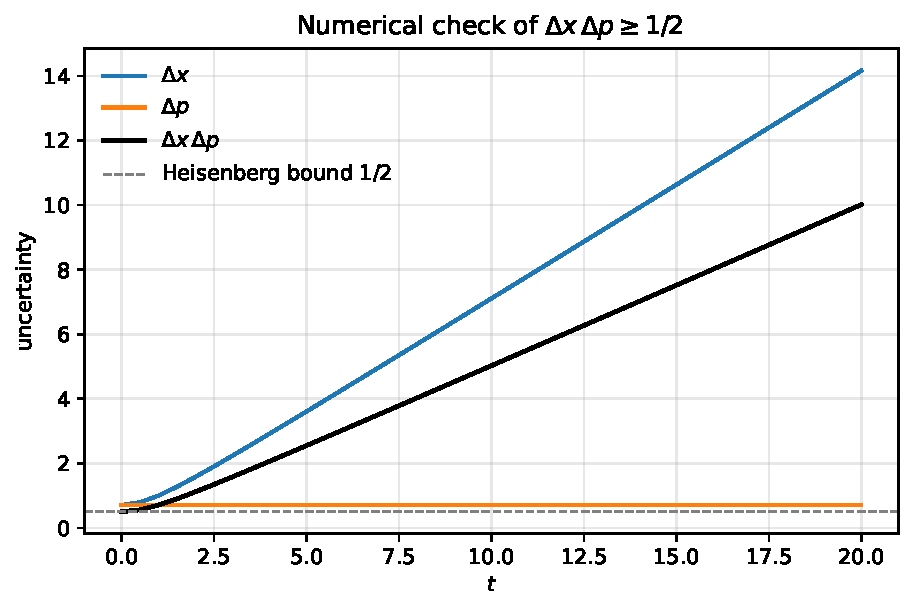
\includegraphics[width=0.75\linewidth]{ch00_uncertainty}
    \caption{$\Delta x(t)$, $\Delta p(t)$ 与乘积 $\Delta x\,\Delta p$ 随时间的变化. 灰色虚线为 Heisenberg 下界 $1/2$. 数值结果显示 $\Delta p$ 严格守恒 (因为 $[\Op H_{0},\Op p]=0$), $\Delta x$ 渐近线性增长, 乘积初值正好饱和 $1/2$ 后单调上升.}
    \label{fig:numexp-ch00-uncert}
\end{figure}

数值输出中前几行为
\begin{verbatim}
t =  0.00  <x> = -10.0000  Dx = 0.7071  <p> = +2.0000  Dp = 0.7071  DxDp = 0.5000
t =  5.00  <x> =  -0.0000  Dx = 3.6056  <p> = +2.0000  Dp = 0.7071  DxDp = 2.5495
t = 10.00  <x> = +10.0000  Dx = 7.1063  <p> = +2.0000  Dp = 0.7071  DxDp = 5.0249
t = 15.00  <x> = +20.0000  Dx = 10.6301  <p> = +2.0000  Dp = 0.7071  DxDp = 7.5166
\end{verbatim}
范数 $\|\psi_{t}\|^{2}$ 在所有时间点均为 $1.000000$, 与 $\Op U_{0}(t)$ 是幺正算符相符.

\subsection*{物理讨论}
\begin{itemize}
    \item \textbf{弥散公式的验证.} 对于初始相干态 Gauss 波包, 解析结果给出 $\Delta x(t)=\sigma\sqrt{1+t^{2}/\sigma^{4}}/\sqrt{2}$. 取 $\sigma=1$ 时, $\Delta x(t)=\sqrt{(1+t^{2})/2}$, 即 $t=0,5,10,15$ 处分别为 $0.7071,3.6056,7.1063,10.6301$, 与表中数值完全吻合, 直接验证了 \eqref{eq:qm-gauss-evolve}.
    \item \textbf{动量分布守恒.} $\Delta p$ 始终为 $1/\sqrt{2}\approx0.7071$. 这是因为 $|\widetilde\psi(p,t)|=|\widetilde\psi(p,0)|$, 自由演化只改变动量分量的相位, 不改变其模——这正是 $\hat\psi(\mathbf p)$ 在驻定相位法 \eqref{eq:qm-asymp-wave} 中保持不变的微观图像.
    \item \textbf{Heisenberg 饱和 \& 失饱和.} 初始 Gauss 是 $\Op x,\Op p$ 的极小不确定态, 故 $\Delta x\,\Delta p|_{t=0}=1/2$ 严格成立; 之后 $\Delta x$ 增大而 $\Delta p$ 不变, 乘积单调增大, 远离下界, 这与一般非定态下的 Robertson 不等式一致.
    \item \textbf{与 Riemann--Lebesgue 引理的呼应.} 图中可以看到, 在任意固定 $x$ 处, $|\psi(x,t)|^{2}$ 随时间趋于 $0$ (波包扫过后高度逐渐降低), 这正是 Riemann--Lebesgue 在弱意义下的体现: $\psi_{t}\rightharpoonup 0$, 但 $\|\psi_{t}\|=1$ 守恒, 故并不是强收敛——这是散射理论中区分 ``在/出态'' 与 ``渐近自由演化'' 的关键技术理由, 在第~\ref{sec:qm-review-summary} 节后续章节将反复用到.
\end{itemize}

\section{本章小结}\label{sec:qm-review-summary}

\begin{itemize}
    \item 散射是探索微观结构的关键工具, 从 Rutherford 到 LHC 都依赖它.
    \item 散射理论分为单道/多道、相对论/非相对论、时间相关/时间无关三对范畴; 本课程聚焦于非相对论、单道(随后会推广到多道)、并交替使用时间相关与时间无关两套语言.
    \item 量子态由 Hilbert 空间中的射线表示; 可观测量对应自伴算符. $L^{2}$ 与 $\ell^{2}$ 是两个具体而典型的可分 Hilbert 空间, 任意无穷维可分 Hilbert 空间都同构于 $\ell^{2}$.
    \item Dirac 记号通过 Riesz 引理把 Hilbert 空间与对偶空间一一联系起来; bra 是有界线性泛函, ket 是矢量.
    \item 线性算符可以是无界的, 因此一定要小心定义域. 厄米共轭对一般算符不一定 ``$A^{\dagger}=A$''; 自伴 (self-adjoint) 算符才有完整谱定理.
    \item 幺正算符要求 $\mathscr D=\mathscr R=\Hilb$, 等价于 $U^{\dagger}U=UU^{\dagger}=I$. Isometric 算符只要求 $\mathscr D=\Hilb$ 且保 norm; 在无穷维空间中, isometric $\not\Rightarrow$ unitary.
    \item 强极限与弱极限: 强极限是物理上有意义的``态相同'', 弱极限太弱; 散射理论中所有极限默认理解为强极限. 一系列幺正算符的强极限只能保证 isometric, 这正是 M\o ller 算符的来源.
    \item 自由演化算符 $\rme^{-\rmi\Op H_0 t/\hbar}$ 在动量空间是逐点相位 \eqref{eq:qm-U0-momentum}; 坐标空间的自由传播子 $K_{0}(\mathbf x,\mathbf x';t)$ 是 Gauss 振荡核 \eqref{eq:qm-free-propagator}, $|K_{0}|\propto|t|^{-3/2}$.
    \item 自由 Gauss 波包随时间线性弥散 \eqref{eq:qm-gauss-evolve}; 任意波包按 Riemann--Lebesgue 引理在每一固定坐标点弱收敛到零, 但范数守恒, 故无强极限.
    \item 驻定相位法给出长时间渐进 \eqref{eq:qm-asymp-wave}: 在 $\mathbf x=\mathbf v t$ 上, 波函数振幅 $\sim|t|^{-3/2}\hat\psi(m\mathbf v)$, 动量分布 $|\hat\psi(\mathbf p)|^{2}$ 守恒——这是 ``经典对应''与散射截面定义的物理依据.
    \item 自由 Green 算符 $\Op G_{0}(z)=(z-\Op H_{0})^{-1}$ 在动量空间为 \eqref{eq:qm-G0-p}, 在坐标空间是球面波 Green 函数 \eqref{eq:qm-G0-x}; $\pm\rmi 0^{+}$ 选择对应外向/内向边界条件, 这是 Lippmann--Schwinger 方程的种子.
\end{itemize}

掌握以上数学工具后, 我们就可以严格定义散射算符 $\Smat$ 与跃迁算符 $\Tmat$, 这是从第~\ref{ch:hilbert}~章 (Hilbert 空间与谱理论) 与第~\ref{ch:Smat1P}~章 (单粒子散射算符) 开始的内容.
